%%%%%%%%%%%%%%%%%%%%%%%%%%%%%%%%%%%%%%%%%
% Programming/Coding Assignment
% LaTeX Template
%
% This template has been downloaded from:
% http://www.latextemplates.com
%
% Original author:
% Ted Pavlic (http://www.tedpavlic.com)
%
% Note:
% The \lipsum[#] commands throughout this template generate dummy text
% to fill the template out. These commands should all be removed when 
% writing assignment content.
%
% This template uses a Perl script as an example snippet of code, most other
% languages are also usable. Configure them in the "CODE INCLUSION 
% CONFIGURATION" section.
%
%%%%%%%%%%%%%%%%%%%%%%%%%%%%%%%%%%%%%%%%%
 
%----------------------------------------------------------------------------------------
%	PACKAGES AND OTHER DOCUMENT CONFIGURATIONS
%----------------------------------------------------------------------------------------

\documentclass{article}

\usepackage{fancyhdr} % Required for custom headers
\usepackage{lastpage} % Required to determine the last page for the footer
\usepackage{extramarks} % Required for headers and footers
\usepackage[usenames,dvipsnames]{color} % Required for custom colors
\usepackage{graphicx} % Required to insert images
\usepackage{listings} % Required for insertion of code
\usepackage{courier} % Required for the courier font
\usepackage{url}
\usepackage{paralist}
\usepackage{pgfgantt}
% Margins
\topmargin=-0.45in
\evensidemargin=0in
\oddsidemargin=0in
\textwidth=6.5in
\textheight=9.0in
\headsep=0.25in

\linespread{1.1} % Line spacing

% Set up the header and footer
\pagestyle{fancy}
\lhead{\hmwkAuthorNameShort} % Top left header
\chead{\hmwkTitle} % Top center head
\rhead{} % Top right header
\lfoot{} % Bottom left footer
\cfoot{} % Bottom center footer
\rfoot{Page\ \thepage\ of\ \protect\pageref{LastPage}} % Bottom right footer
\renewcommand\headrulewidth{0.4pt} % Size of the header rule
\renewcommand\footrulewidth{0.4pt} % Size of the footer rule

%\setlength\parindent{0pt} % Removes all indentation from paragraphs

%----------------------------------------------------------------------------------------
%	CODE INCLUSION CONFIGURATION
%----------------------------------------------------------------------------------------
\definecolor{mygreen}{rgb}{0,0.6,0}
\definecolor{mygray}{rgb}{0.5,0.5,0.5}
\definecolor{mymauve}{rgb}{0.58,0,0.82}

\lstset{ %
  backgroundcolor=\color{white},   % choose the background color; you must add \usepackage{color} or \usepackage{xcolor}
  basicstyle=\footnotesize,        % the size of the fonts that are used for the code
  breakatwhitespace=false,         % sets if automatic breaks should only happen at whitespace
  breaklines=true,                 % sets automatic line breaking
  captionpos=b,                    % sets the caption-position to bottom
  commentstyle=\color{mygreen},    % comment style
  deletekeywords={...},            % if you want to delete keywords from the given language
  escapeinside={\%*}{*)},          % if you want to add LaTeX within your code
  extendedchars=true,              % lets you use non-ASCII characters; for 8-bits encodings only, does not work with UTF-8
  frame=single,                    % adds a frame around the code
  keepspaces=true,                 % keeps spaces in text, useful for keeping indentation of code (possibly needs columns=flexible)
  keywordstyle=\color{blue},       % keyword style
  language=Octave,                 % the language of the code
  morekeywords={*,...},            % if you want to add more keywords to the set
  numbers=left,                    % where to put the line-numbers; possible values are (none, left, right)
  numbersep=5pt,                   % how far the line-numbers are from the code
  numberstyle=\tiny\color{mygray}, % the style that is used for the line-numbers
  rulecolor=\color{black},         % if not set, the frame-color may be changed on line-breaks within not-black text (e.g. comments (green here))
  showspaces=false,                % show spaces everywhere adding particular underscores; it overrides 'showstringspaces'
  showstringspaces=false,          % underline spaces within strings only
  showtabs=false,                  % show tabs within strings adding particular underscores
  stepnumber=2,                    % the step between two line-numbers. If it's 1, each line will be numbered
  stringstyle=\color{mymauve},     % string literal style
  tabsize=2,                       % sets default tabsize to 2 spaces
  title=\lstname                   % show the filename of files included with \lstinputlisting; also try caption instead of title
}


\newcommand{\includecode}[2]{\lstinputlisting[caption=#2,captionpos=t,language=C]{code/#1}}


%----------------------------------------------------------------------------------------
%	NAME AND CLASS SECTION
%----------------------------------------------------------------------------------------

\newcommand{\hmwkTitle}{Nios Code Generation Specification} % Assignment title
\newcommand{\hmwkDueDate}{\today} % Due date
\newcommand{\hmwkClass}{} % Course/class
\newcommand{\hmwkClassTime}{} % Class/lecture time
\newcommand{\hmwkClassInstructor}{} % Teacher/lecturer
\newcommand{\hmwkAuthorName}{Jonah Caplan} % Your name
\newcommand{\hmwkAuthorNameShort}{Caplan} % Your name

%----------------------------------------------------------------------------------------
%	TITLE PAGE
%----------------------------------------------------------------------------------------

\title{
\vspace{2in}
\textmd{\textbf{\hmwkTitle}}\\
\vspace{3in}
}

\author{\textbf{\hmwkAuthorName}}
\date{} % Insert date here if you want it to appear below your name



%----------------------------------------------------------------------------------------

\begin{document}

\maketitle
\thispagestyle{empty}
\newpage
\setcounter{page}{1}

%------------------------------------------------------------------------------------
\section{Introduction}

The aim of this project is to develop an infrastructure for the automatic generation of C code for multicore Nios systems. We assume that an external model based design approach is used to generate control algorithms and that C code for these computations have already been generated in separate files (e.g. Simulink). The purpose of this tool is to efficiently map the control system onto an arbitrary platform while taking into account non-functional requirements such as deadlines, data flow, and criticality. The user must only specify the requirements for the system at a high level of abstraction and all intermdeiate code will be automatically generated. 

This tool will not initially be geared towards solving codesign problems. We will assume a static hardware platform and ocnsider changing software requirements only. In order to facilitate later expansions, the tool will require the specification of the hardware in terms of generic model parameters. The task-mapping procedure will be platform independent and solve the problem generically even if we do not currently take advantage of this feature.

This document will provide the specification for the currently supported hardware models, the platform built from these components currently under study, the application models for analysis of software requirements, the mapping procedure combining both hardware and software models to generate a schedule, and the abstract template requirements for code generation.



%%%%%%%%%%%%%%%%%%%%%%%%%%%%%%%%%%%%%%%%%%%%%%%%%%%%%%%%%%%%%%%%%%%%%%%%%%%%%%%%%%%%%%%%%%%%%%%%%%%%%%%%%%%%%%%%
\section{Tool Structure}

This key to success for this project in the given time frame is to leverage open source, take advantage of the wealth of prior work in the field from the 1990s in synchronous language design, and more current work on automated DSE and code generation. Furthermore, the wealth of generated code that describes the platform, as well as a very well structured RTOS uC/OS-II integrated into the BSP make the job of template development and hardware platform specification much easier. While the code can be a bit cumbersome to navigate for a human user because it is generated, this actually makes it much easier to parse for an automated process.


Figure \ref{f:tool_arch} depicts the tool architecture. From this figure we can begin to derive a timeline for development by identifying and prioritizing milestones. Figure \ref{f:gantt} depicts an equivalent Gantt chart.

\begin{enumerate}
\item Define model classes for application and processors.
\item Integrate models with GA library to build task mapper.
\item Test mapper extensively with randomly generated task graphs, including timing data and fault-tolerance requirements.
\item Write RTOS templates.
  \begin{enumerate}
  \item Deconstruct existing code into discrete units with well-defined functionality.
  \item Formalize inter-core communication protocols.
  \item Write new templates for non-existing features (e.g. killing erroneous tasks, setting MPU parameters).
  \item Rewrite all drivers for fingerprint unit, comparator and TLB.
  \end{enumerate}
\item Build code generation tool.
\item Port Heptane from MIPS to Nios architecture.
\item Define QSYS naming conventions and write system.h BSP parser.
\item Write language specification for high level model input.
\item Write scanner/parser using SableCC3 to build abstract Java application model from user input. 
\end{enumerate}




% \newpage


\begin{figure}[h]
\centering
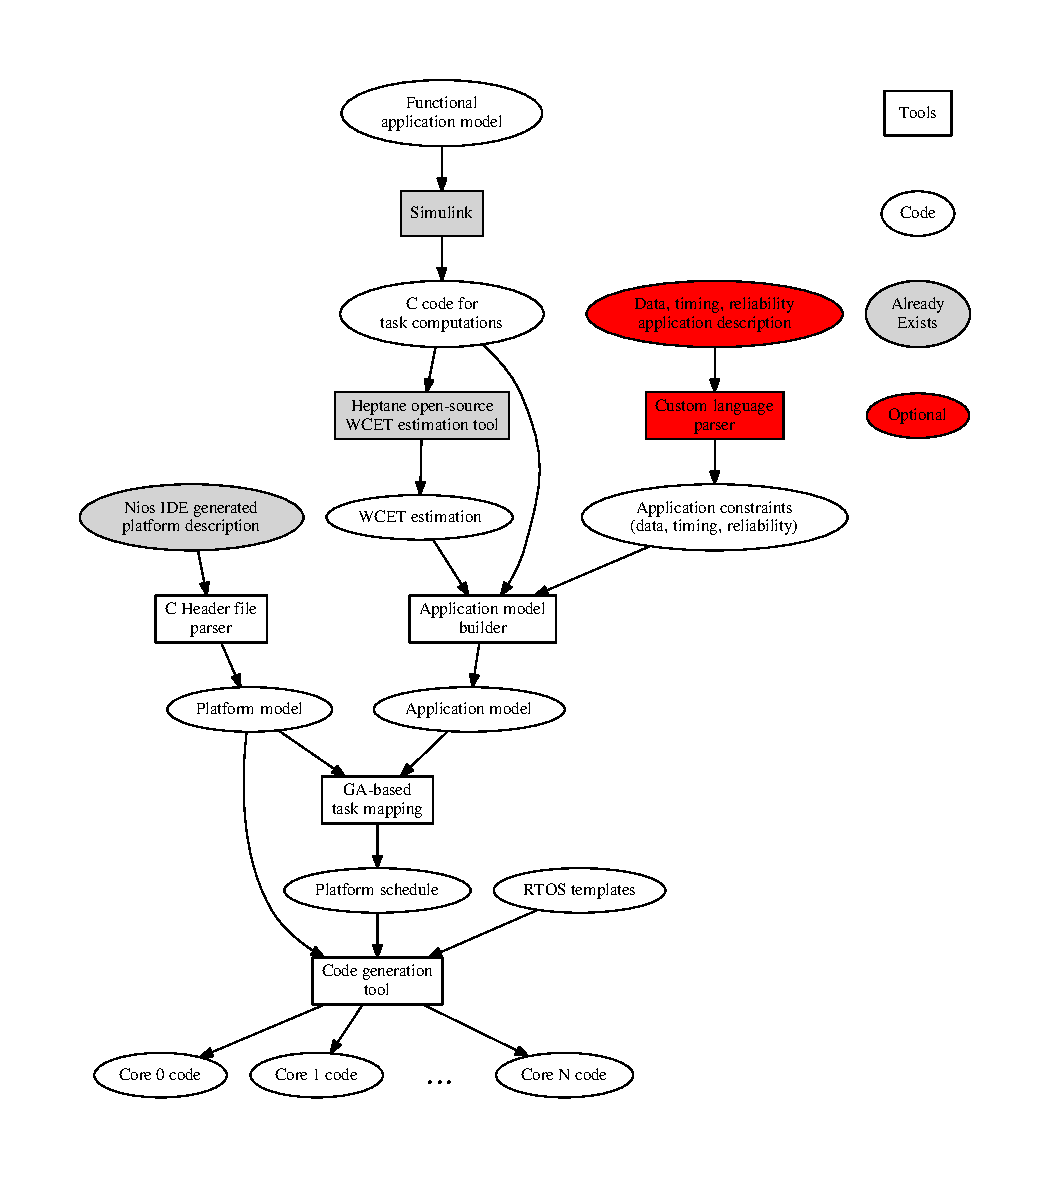
\includegraphics[scale=0.8]{figures/tool_arch}
\caption{The proposed tool architecture.}
\label{f:tool_arch}
\end{figure}


\begin{figure}[h]
% \begin{center}
\begin{ganttchart}{1}{8}
% \gantttitle{Development Timeline}{8} \\
\gantttitlelist{1,...,8}{1} \\
\ganttbar{Define Model Classes}{1}{1} \\
\ganttlinkedbar{Build task mapper}{2}{2} \\
\ganttlinkedbar{Write RTOS templates}{3}{3} \\
\ganttlinkedbar{Code generation tool}{4}{4} \\
\ganttlinkedbar{Port Heptane}{5}{5} \\
\ganttlinkedbar{Nios BSP parser}{6}{6} \\
\ganttlinkedbar{Specify application modelling language}{7}{7} \\
\ganttlinkedbar{Scanner/Parser for modelling language}{8}{8} \\
% \ganttgroup{Group 1}{1}{7} \\
% \ganttlinkedbar{Task 2}{3}{7} \ganttnewline
% \ganttbar{Final Task}{8}{12}

\end{ganttchart}
% \end{center}
\caption{Timeline for development of main tool components}
\label{f:gantt}
\end{figure}

%%%%%%%%%%%%%%%%%%%%%%%%%%%%%%%%%%%%%%%%%%%%%%%%%%%%%%%%%%%%%%%%%%%%%%%%%%%%%%%%%%%%%%%%%%%%%%%%%%%%%%%%%%%%%%%%
\section{Hardware Model}
Hardware models are specified using an object-oriented semantics. The system is divided into hierarchical levels that are interpreted using static scoping rules to aid in the specification of larger models. 

The cost in tiucme of transmitting over communication channel models is omitted at this stage beyond specifying the connections between elements. Issues related to resource arbitration and interference are also not considered. The underlying infrastructure is assumed to be sufficiently quick and deterministic.

There are four categories of hardware models in the system: processor cores, peripheral cores, and memory and buses.

\subsection{Processor cores}
All processor cores are assumed to operate at the same clock frequency. Their parameters are determined during hardware design and are not altered during software mapping. They can be extracted from the \emph{system.h} file generated from the {.sopcinfo} file by the Nios IDE during BSP generation.

Processor parameters are:
\begin{enumerate}
\item \emph{Fault-tolerant}: While we do not have access to safety-critical Nios licenses, they do exist. We assume that a core can be designated as fault tolerant (FT) and that a cost is associated with fault tolerance (due to licensing, size, resource utilization, power consumption as appropriate for the scenario) and that it is therefore necessary to have fewer FT cores in the system.

\item \emph{Scratchpad}: 
The processor must have a scratchpad in order to use fingerprinting as an error detection mechanism under our current implementation. The relevant parameters for the scratchpad will be listed separately.

\item \emph{Timer}: 
The system timer will dictate the minimum period for events in the system. The timer period is statically assigned when specifying the hardware design in QSYS.

\item \emph{Fingerprint Unit}: 
Fingerprint units will be necessary to allow the monitoring of processing cores (PC), i.e. those cores lacking FT capabilities, by a FT core.
 
\item \emph{Data and instruction cache}: 
It may be necessary to disable data and/or instruction caches while executing critical tasks. It must be known if the processor is equipped with either.

\item \emph{DMA}:
A single channel DMA will be used to shuttle critical data in and out of the scratchpads.

\item \emph{MPU}:
An MPU will be required to ensure that each core is unable to maintain partitions between each core.

\item \emph{Shared memory}:
Shared memory space will be required to load instructions

\item \emph{Interrupt signals}:
The processor model must specify the actively connected interrupt signals.

\end{enumerate}

This is a very general model of the processor. The mapping of tasks to cores will take place considering a very high level model of the system. The lower level parameters will only be used for code generation purposes. For the processor model, it is sufficient to consider whether or not each of these components are available. The details of each component will be hidden from the mapping problem at this higher level of abstraction.

\subsection{Memory}
Local scratchpads will be required for each core as well as shared main memory. A memory is defined simply as a start and end address. Memory latencies are not modelled. A memory model will also keep track of what other modules are connected to it.

There will be two partitioned sections of shared main memory. One to access common functions for redundant task executions and another for message passing between cores.

\subsection{Peripherals}
Certain details about the peripherals such as control registers will be entirely encapsulated in the template objects for the code generation phase. The higher level concerns that will dictate how these registers are sit will be included in the object representation of each peripheral. Mappings from the higher level concerns to code generation rules will be specified.

\subsubsection{Timer}
The frequency of the system level timer must be known in order to define the minimum resolution of time in the application model. Preexisting drivers exist and macros are generated by the Nios IDE to manage the timer. All relevant macros can be extracted from the generated code.

\subsubsection{Fingerprint Unit} 
The fingerprint unit has the following features: maximum stack depth, statically set during hardware design, and block length size. The setting of

\subsubsection{Memory Protection Unit}

\subsubsection{Comparator}

\subsubsection{DMA}

\subsubsection{$\mu$TLB}


%%%%%%%%%%%%%%%%%%%%%%%%%%%%%%%%%%%%%%%%%%%%%%%%%%%%%%%%%%%%%%%%%%%%%%%%%%%%%%%%%%%%%%%%%%%%%%%%%%%%%%%%%%%%%%%%

\section{Application Model}
\subsection{Synchronous Languages - Building off the past}

\subsection{Code Rules}
Any data passed between tasks must be done through pointers. Functions will return void pointers to predetermined data structures. These pointers will be passed between tasks. If tasks cannot share the same memory space, then the size of the data structure must also be known and the data will be copied to the appropriate location.


%%%%%%%%%%%%%%%%%%%%%%%%%%%%%%%%%%%%%%%%%%%%%%%%%%%%%%%%%%%%%%%%%%%%%%%%%%%%%%%%%%%%%%%%%%%%%%%%%%%%%%%%%%%%%%%%

\section{Code Profiling}
 
The disassembly of a simple benchmark that runs the main computation loop will be parsed to analyse code to estimate the WCET and maximum stack height of each critical task. All functions that are called by the critical task will be identified in order to partition code through linker script modifications, thus enabling the use of instruction scratchpads.


%%%%%%%%%%%%%%%%%%%%%%%%%%%%%%%%%%%%%%%%%%%%%%%%%%%%%%%%%%%%%%%%%%%%%%%%%%%%%%%%%%%%%%%%%%%%%%%%%%%%%%%%%%%%%%%%
\section{Application Mapping}

The initial scheduling algorithm will be taken from Bolchini and  Miele \cite{bolchini2013reliability}. A genetic algorithm (GA) is used to explore the design space. The general details that follow on genetic algorithms are based on the overview in \cite{geatbx}.

Figure \ref{f:ga_ov} shows an overview of how to implement a genetic algorithm. There are two stages of GA in the given process. First tasks must be organized into groups of tasks, and each group of tasks must be assigned a fault detection technique or fault tolerance technique. DMR Fingerprinting is an example of a detection mechanism. This work will remain agnostic about the method of implementation of fault tolerance. We assume that appropriate hardening measures are applied to a single core.

\begin{figure}[h]
\centering
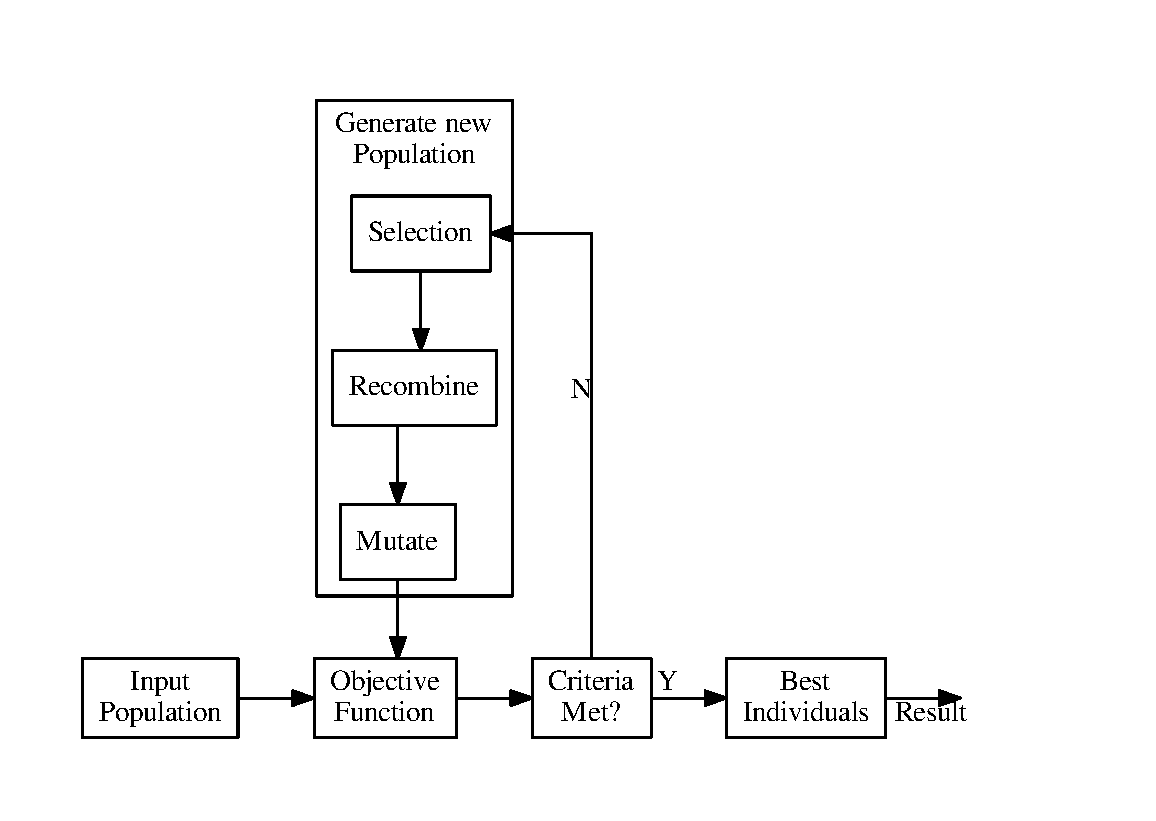
\includegraphics[width=12cm]{figures/ga_ov}
\caption{The basic structure of a genetic algorithm \cite{geatbx}.}
\label{f:ga_ov}
\end{figure}

Once a population of various groupings and associated fault-handling mechanisms has been generated it is necessary to test their fitness. This must be done by generating a system schedule for each member of the population. 

The generation of the schedule is itself done with a second round of GA. Each task is assigned to an appropriate core based on the fault-handling requirements of its group. The group adopts the most stringent requirements of any of its members. Various mappings are generated as the GA population. Then it is necessary to order the tasks on each core. This is complicated by the fact that there may be inter-core data dependencies. For now, we will neglect the overhead associated with data transfer between cores.

The first step for scheduling on each core once groups have been assigned is to generate a list of tasks for which all the start conditions have been met (i.e. data dependencies on previously executed tasks). The highest priority task is chosen from this list for each core. This process cycles through all the cores and then proceeds to the next event in time (i.e. a task has ended) to repeat the process. 

The priority of a task is determined using \emph{modified partial critical path priority} \cite{eles2000scheduling}. The method consists of choosing tasks that minimize the critical path on \emph{other cores}. It is possible that a successor to a task will be in the pool of tasks. Therefore, the critical path length is only considered from the first successor task that will execute on a different core. 

Consider the example from \cite{eles2000scheduling} in Figure~\ref{f:crit_path}. From a start point $P_0$, either task $P_A$ or $P_B$ must be selected. The chain of tasks from $P_A$ to $P_X$ represents a series of successor tasks that will all be executed on the same core in time $t_A$. The time $\lambda_A$ represents the time from the first successor on a different core to the terminal or sink task $P_N$. The scheduler must determine whether to assign $P_A$ or $P_B$ higher priority. This is done by choosing the option that minimizes the critical path \emph{on other cores}. This means that $t_A$ and $t_B$ are neglected and the path with shorter $\lambda$ is chosen. One interesting question is whether it would be simpler and more effective on a system with \emph{many} cores to simply choose the task with the largest number of critical children nodes or non-critical children nodes (in that order) since this will most likely facilitate parallel execution on a large system.

\begin{figure}[h]
\centering
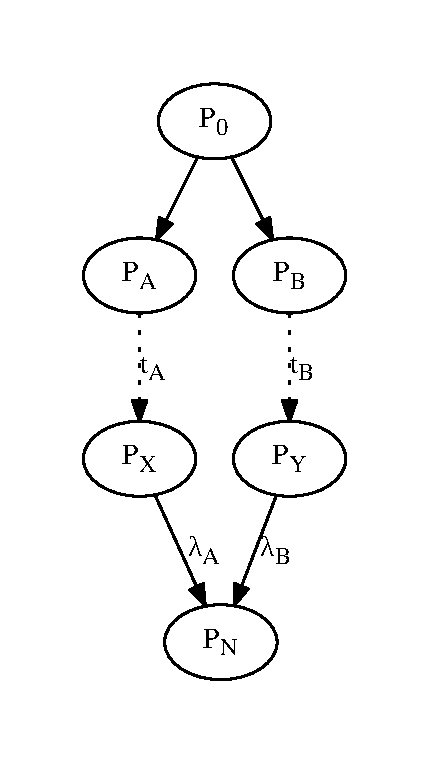
\includegraphics[scale=0.7]{figures/crit_path}
\caption{Example of modified partial critical path priority selection \cite{eles2000scheduling}.}
\label{f:crit_path}
\end{figure}



The implementation details of the genetic algorithm will be adopted from \cite{bolchini2013reliability}. Tournament selection and single-point crossover operator recombination will be used. Mutations will be applied randomly. There are four mutations at the task level: change the group of a task, split a group in two, join two groups, or change the fault-management technique applied to a group. The mutation for the mapping phase consists of switching a task to another processor that can meet the assigned fault-management requirements.

Tournament selection means choosing a subset of the population and selecting the most fit member. This is repeated as many times as necessary. Single-point crossover cuts two parent chromosomes into two pieces and then exchanges the second substrings between the chromosomes. 

The initial parameters for the GA will be the ones suggested in \cite{bolchini2010multi}. The crossover rate is 80\%, the mutation rate is 10\%. The program will run for 30 generations. The population size will be between one and two thousand.

The JGAP library \cite{jgap} is used to implement the genetic algorithm. 

\subsection{Recovery}
Fault model: can't fail twice.
Need to leave room for reexecution. 
Fill up the retry slots with soft tasks. Just cancel them if the retry slot is needed.

Recovery only necessary in the case of correction. Detection implies no retry. 

Why? Application where delivering the wrong answer can be catastrophic but dropping a frame is acceptable (i.e. not sensitive to jitter)



%%%%%%%%%%%%%%%%%%%%%%%%%%%%%%%%%%%%%%%%%%%%%%%%%%%%%%%%%%%%%%%%%%%%%%%%%%%%%%%%%%%%%%%%%%%%%%%%%%%%%%%%%%%%%%%%
\section{Code Generation}

Code generation will be decomposed into several phases.



\bibliographystyle{ieeetr}
\bibliography{codegen}


\end{document}